% !TEX root = ../main.tex

%----------------------------------------
%   SECTION TITLE
%----------------------------------------
\chapter{User Interface}
\label{chap:user_interface}
%----------------------------------------
%   SECTION CONTENT
\section{Components}
In TEASync, UI components are written as a combination of geometric shapes. Generation of components dynamically is also possible, and updates to component attributes can be associated with the local and global models. Although these components lack native HTML API support, this approach can be useful to viewers who are not familiar with HTML and CSS to create components.


An example of a component for Calendar application is below.

\begin{lstlisting}[language=Haskell, caption=Defining a shape component in TEASync., label=lst:java]
grip = [ wedge 5 0.5
       |> filled yellow 
       |> rotate (degrees 90)
   , line (-4,1.25) (4,1.5) |> outlined (solid 0.5) (rgb 150 150 0)    
   , line (-3,2.5) (3,2.5) |> outlined (solid 0.5) (rgb 150 150 0)    
   , line (-1,3.75) (1,3.75) |> outlined (solid 0.5) (rgb 150 150 0)    
   ]
     |> group
\end{lstlisting}

For React application, we used an UI component library[3], \lstinline{shadcn}, to add the customization button and dialog boxes in our application. These components support native HTML API. In addition to the component library, the Tailwind\cite{tailwindcss} CSS framework helps customize the look and feel of the application [5]. These additions helped to create a responsive UI for mobile and desktop clients, avoiding boilerplate code to a very large extent. 

Below, we show an example of a React component for a chatroom application.

\begin{lstlisting}[language=Haskell, caption=Defining a component in React., label=lst:java]
export default function MessageInput({send}) {
    return (
        <div className="h-1/6 bg-blue-400 flex p-2 space-x-1">
            <form className="flex basis-full space-x-1" action={send}>
                <input name="message" className="basis-5/6 placeholder:italic" placeholder="type..." type="text" />
                <button type="submit" className="basis-1/6 bg-green-800 w-1/6 h-full rounded text-fuchsia-100">Send</button>
            </form>
        </div>
    )
}
\end{lstlisting}

When comparing with TEASync, one can modify the look and feel of the components while describing the component or loading components from other modules. As currently TEASync does not support any CSS framework or component library, significant effort is required to create professional looking components with animations and other features. 



\section{Drag-n-Drop}
Building drag-n-drop components in web applications can be challenging, especially when aiming to deliver a seamless and intuitive user experience. Few of these challenges include cross-browser compatibility, event handling and coordination, drop target detection and validation, etc. Building an application from scratch where the user can seamlessly drag-and-drop events across the calendar comes with such challenges.

In the Calendar application, one requirement was that users must be able to drag and drop the events in the calendar across the view. When an event is dragged and dropped, the Calendar application should update its attributes, such as start/end time and date.

The TEASync application implements the drag-and-drop feature from scratch and dynamically adds draggable components. The following code shows the implementation of the calendar component, which includes the reacting to the user event of grabbing and dragging components across the view.

\begin{lstlisting}[language=Java, caption=TEASync Calendar Shape, label=lst:java, mathescape=true]
    myShapes localModel globalModel =
  [
    Debug.toString localModel |> text |> size 4 |> filled black |> move (-90,60)
  , Debug.toString globalModel |> text |> size 4 |> filled black |> move (-90,56)
  ]
  ++
  ( List.indexedMap ( \ idx day -> 
                        [ rect dayWidth 100 |> outlined (solid 0.5) black
                            |> move (dayWidth * toFloat idx - 2*dayWidth, 0)
                        , text day |> size 4 |> centered |> filled black 
                            |> move (dayWidth * toFloat idx - 2*dayWidth, 45)
                        ]
                          |> group
                            
             )
             ["Monday","Tuesday","Wednesday","Thursday","Friday"]
  )
  ++
  [ case localModel.dragState of
      Waiting -> rect (dayWidth*5) 100 |> filled (rgba 0 0 0 0)
                    |> notifyMouseDownAt (MouseDownToAddMeetingAt >> LocalMsg)
      _ -> group []
  ]
  ++
  ( globalModel.calendar |> Dict.toList 
      |> List.map ( \ (dayStart, meeting) -> drawMeeting dayStart meeting False ) 
  )
  ++
  ( case localModel.dragState of
      Waiting -> []
      DraggingStart dayStart dragDayTime meeting -> 
        [ drawMeeting dragDayTime meeting True
        , rect (dayWidth*5) 100 |> filled (rgba 0 0 0 0)
          |> notifyMouseMoveAt (MouseMoveAt >> LocalMsg)
          |> notifyMouseUp (MouseUp |> LocalMsg)
          |> notifyLeave (MouseUp |> LocalMsg)
          |> notifyMouseUpAt (AddMeetingAt meeting >> GlobalMsg)
          |> notifyMouseUpAt (ChangeMeetingStart dayStart meeting >> GlobalMsg)
        ]
      DraggingEnd   dayStart dragDayTime meeting -> 
        [ drawMeeting dayStart (updateDuration dayStart meeting dragDayTime) True
        , rect (dayWidth*5) 100 |> filled (rgba 0 0 0 0)
          |>  notifyMouseMoveAt (MouseMoveAt >> LocalMsg)
          |> notifyMouseUp (MouseUp |> LocalMsg)
          |> notifyLeave (MouseUp |> LocalMsg)
          |> notifyMouseUpAt (ChangeMeetingEnd dayStart meeting >> GlobalMsg)
        ]
  )
\end{lstlisting}


The React application uses \lstinline{react-big-calendar}\cite{bigcalendar} along with addon \lstinline{dragAndDrop} to build the calendar application. These libraries provide customization options such as localization, default view- week, month, day, look and feel customization, etc. With a few modifications, we could utilize this library to suit our needs. Following is the implementation of the \lstinline{react-big-calendar} along with \lstinline{dragAndDrop} in our React application.


\begin{lstlisting}[language=Java, caption=Drag and Drop Calendar Initialization, label=lst:java, mathescape=true]
import { Calendar, momentLocalizer, Event, Views } from 'react-big-calendar';
import withDragAndDrop from 'react-big-calendar/lib/addons/dragAndDrop';
import moment from 'moment';
import { useSocket } from '/app/SocketProvider';

const localizer = momentLocalizer(moment)
const DnDCalendar = withDragAndDrop(Calendar);

interface MyEvent extends Event {
    title: string;
    resourceId: string;
}
export default function Page({ params }: { params: { id: string } }) {
...
    return (
        ...
            <DnDCalendar
                    localizer={localizer}
                    events={events}
                    selectable='true'
                    onSelectSlot={onSelectSlot}
                    defaultView='week'
                    views={['week']}
                    draggableAccessor={(event) => true}
                    startAccessor="start"
                    endAccessor="end"
                    onView={onView}
                    onNavigate={onNavigate}
                    resizable={true}
                    onEventResize={resizeEvent}
                    onEventDrop={resizeEvent}
                />
        ...
    );
}
\end{lstlisting}

After importing the required features from the library, we initialize the localizer and assign functions to various hooks such as \lstinline{defaultView}, \lstinline{onEventResize}, \lstinline{onEventDrop} etc. DnDCalendar receives a list of \lstinline{events} as input which it renders on the calendar. The \lstinline{resizeEvent} function handles user input and reacts to actions such as resizing or dragging an event to different times or days of the week.

\section{Chatroom Application}

\textbf{TEASync}


% \begin{figure}
%     \centering
%     \includegraphics{}
%     \caption{Caption}
%     \label{fig:enter-label}
% \end{figure}


\begin{figure}[H]
    \centering
    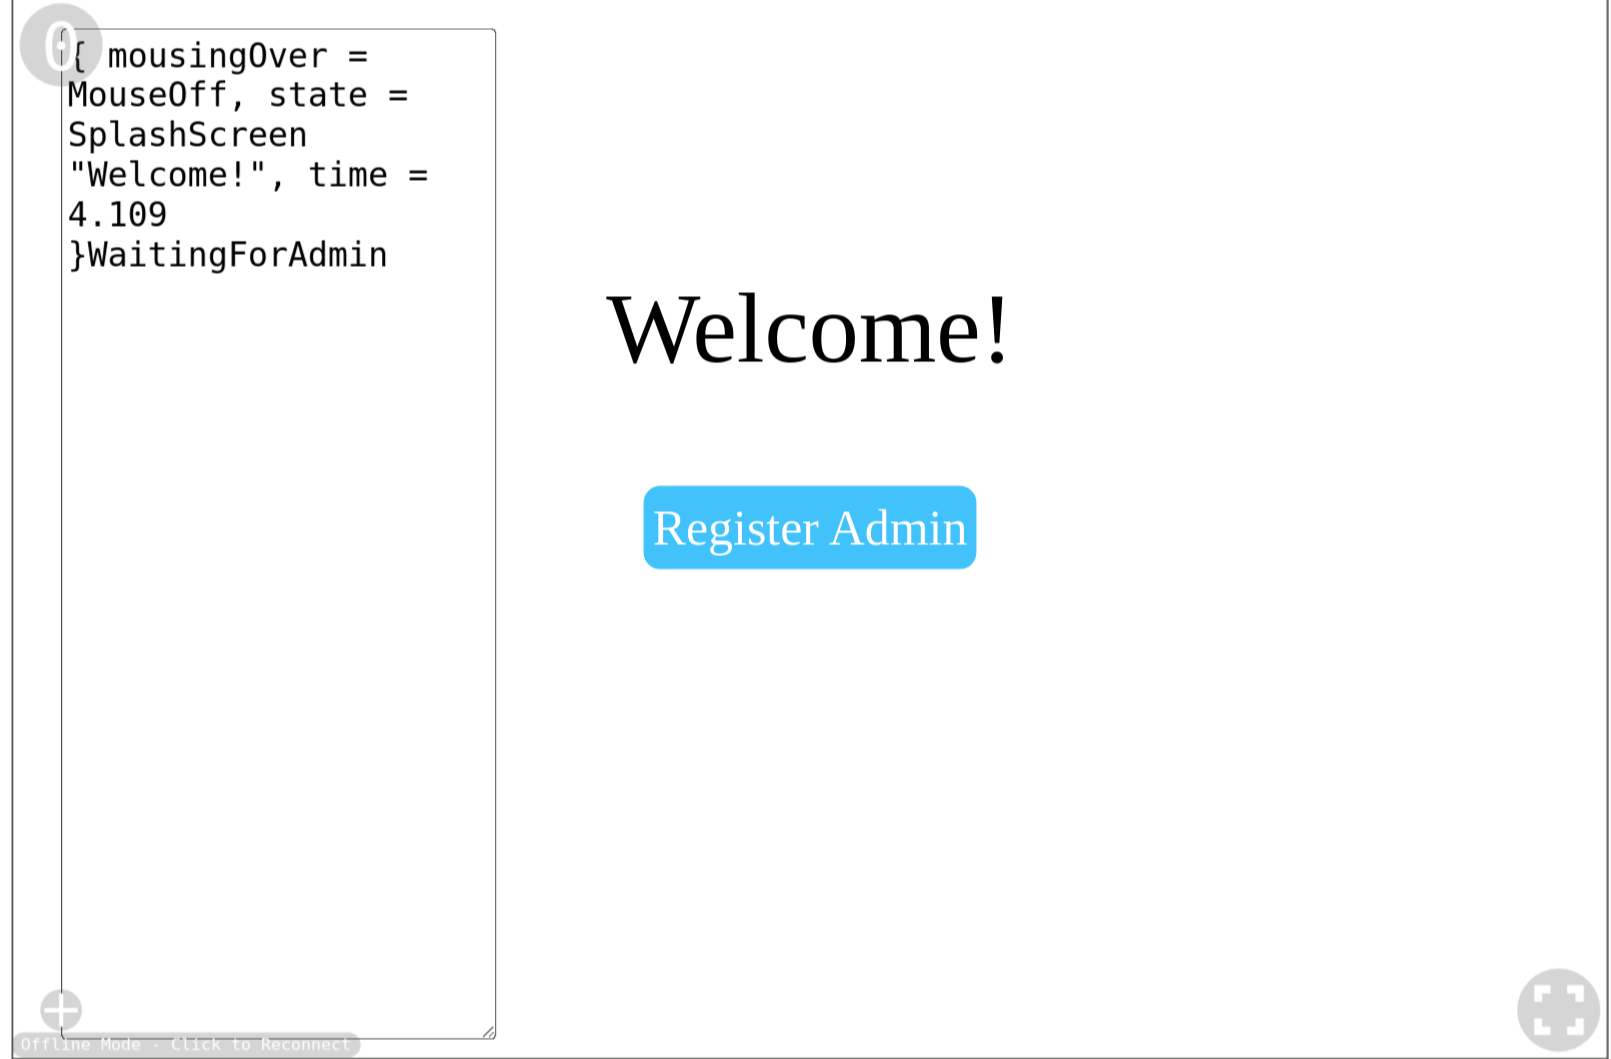
\includegraphics[width=0.8\textwidth]{diagrams/TEASyncChatroomHome.png}
    \caption{TEASync Chatroom: Home Page}
    \label{fig:enter-label}
\end{figure}

\begin{figure}[H]
    \centering
    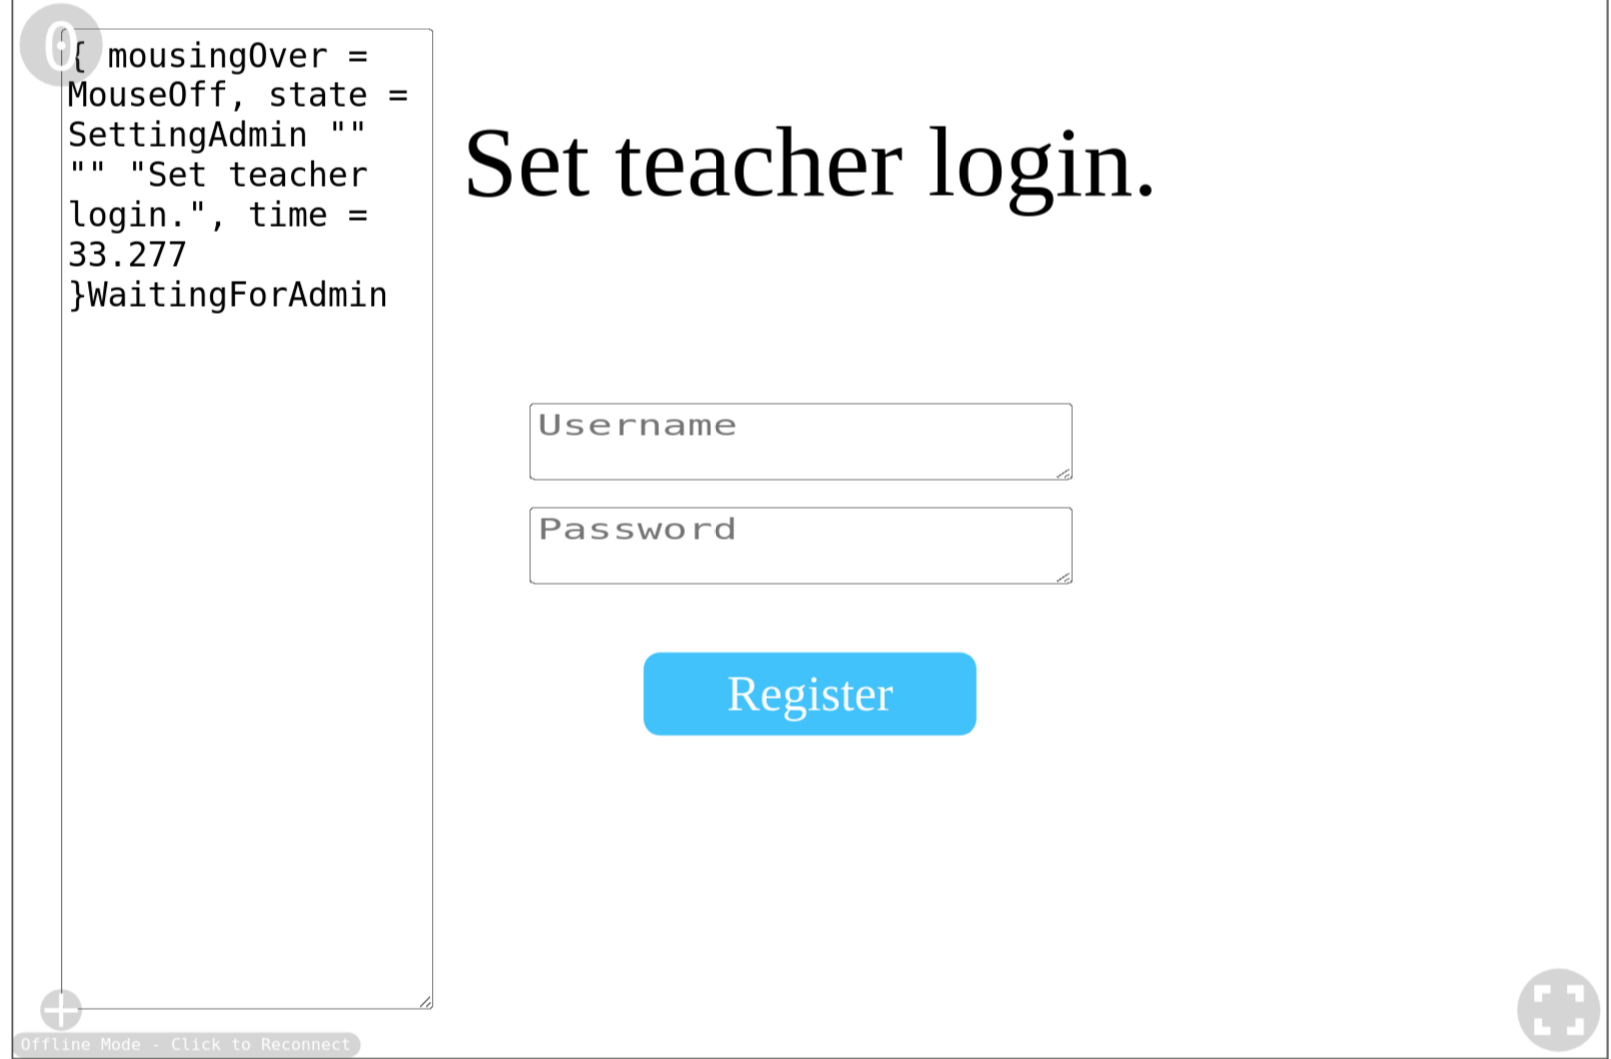
\includegraphics[width=0.8\textwidth]{diagrams/TEASyncChatroomAdminLogin.png}
    \caption{TEASync Chatroom: Admin Login Page}
    \label{fig:enter-label}
\end{figure}

\begin{figure}[H]
    \centering
    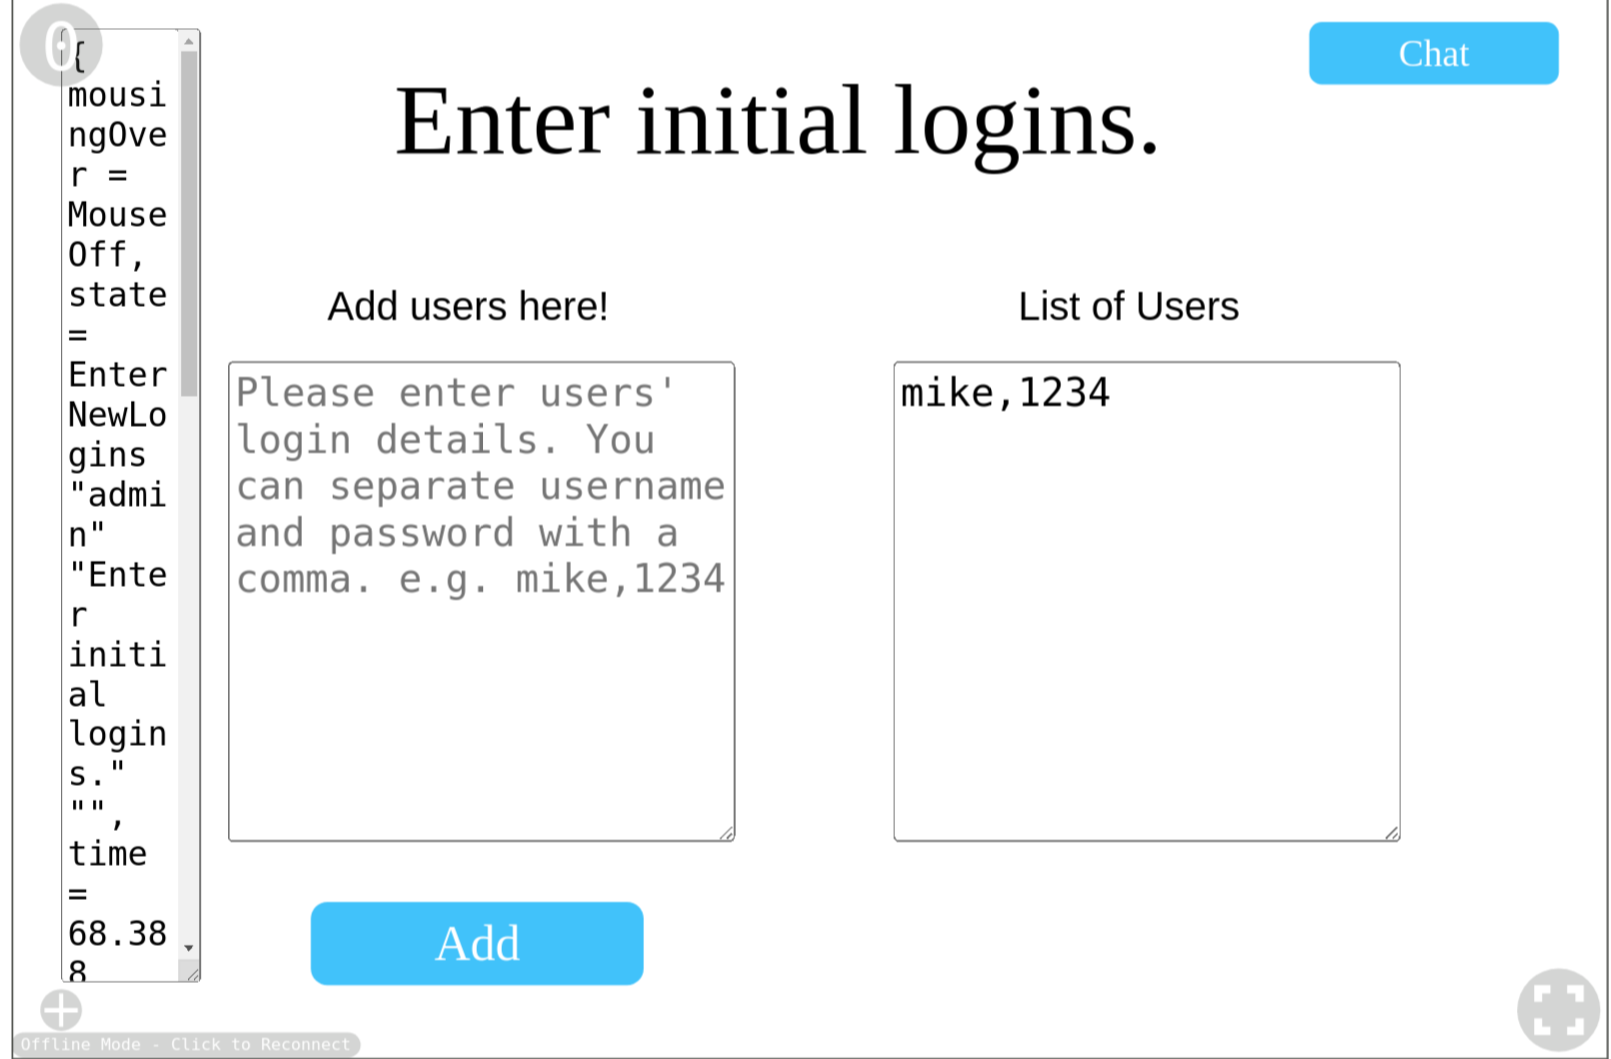
\includegraphics[width=0.8\textwidth]{diagrams/TEASyncChatroomCredsSetup.png}
    \caption{TEASync Chatroom: Credential Setup Page}
    \label{fig:enter-label}
\end{figure}


\begin{figure}[H]
    \centering
    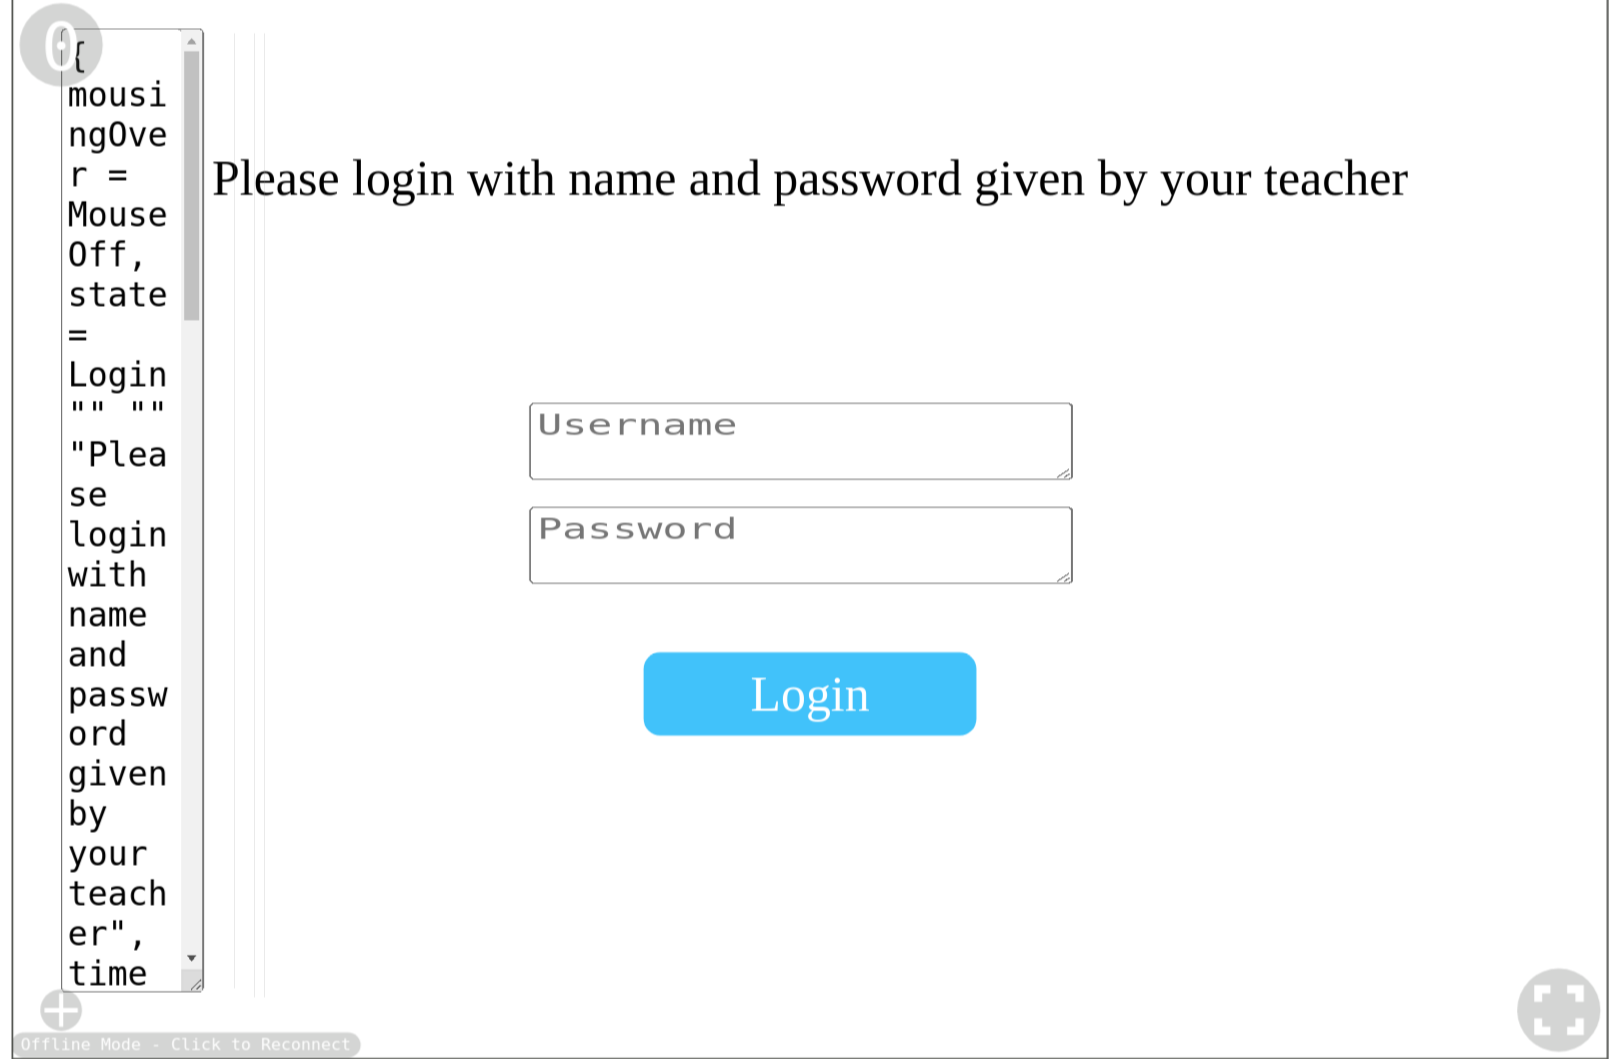
\includegraphics[width=0.8\textwidth]{diagrams/TEASyncChatroomUSerLogin.png}
    \caption{TEASync Chatroom: User Login Page}
    \label{fig:enter-label}
\end{figure}


\begin{figure}[ht]
    \centering
    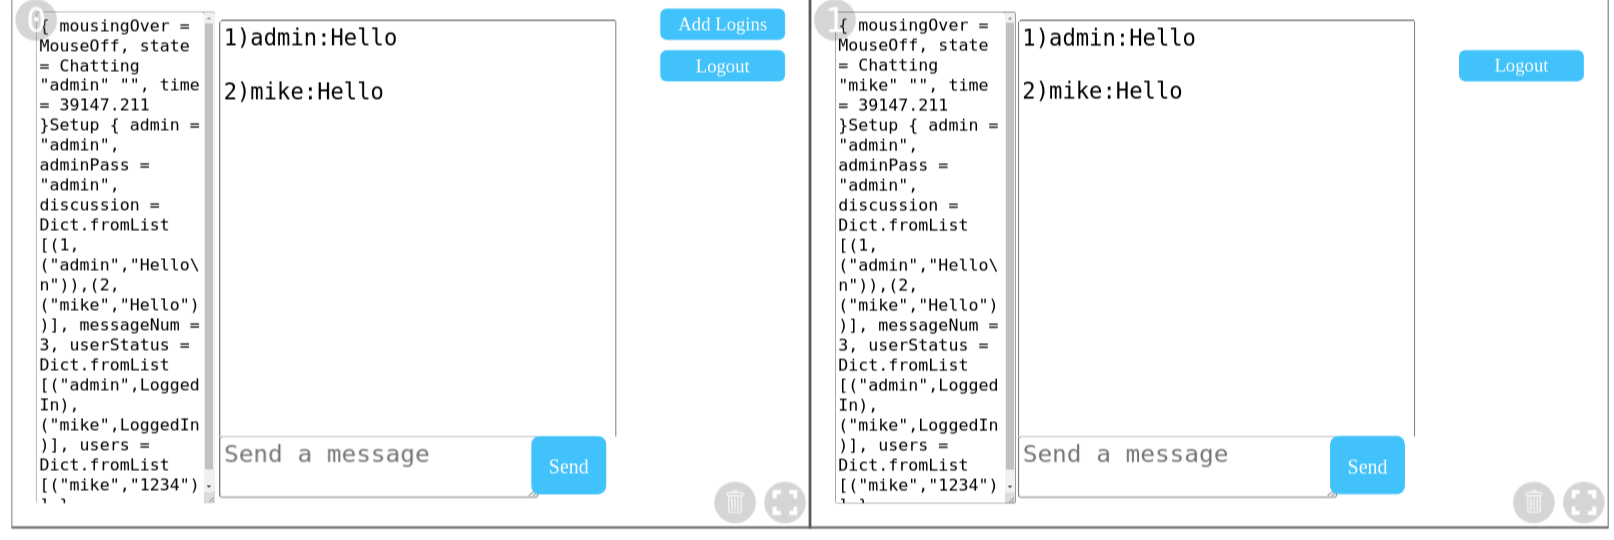
\includegraphics[width=0.8\textwidth]{diagrams/ChatroomMainMultiView.png}
    \caption{TEASync Chatroom: Chat View Page}
    \label{fig:enter-label}
\end{figure}


\textbf{React}

The Chatroom application consists of four main views. The application's homepage is a login view for the admin users to start a session.
\begin{figure}[H]
    \centering
    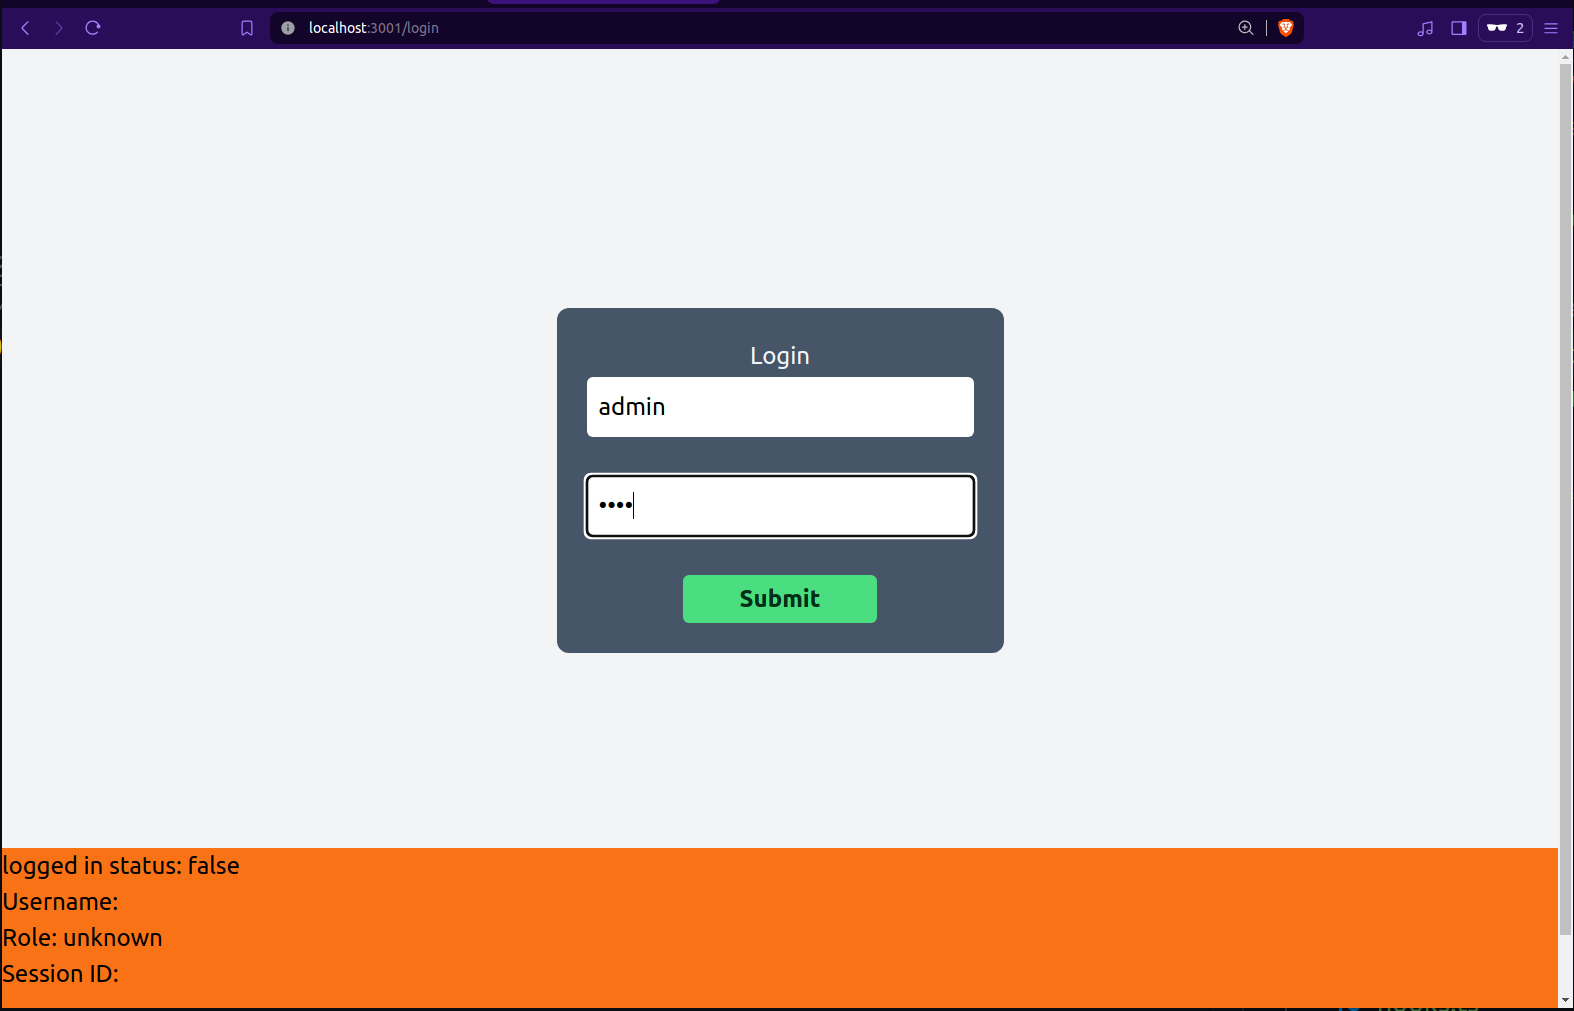
\includegraphics[width=0.8\textwidth]{diagrams/ChatroomAdminLogin.png}
    \caption{React Chatroom: Admin Login Page}
    \label{fig:enter-label}
\end{figure}

After login, admins will be redirected to the new page to create a session. On this screen, admins can enter the users’ details so they can join the session.

\begin{figure}[H]
    \centering
    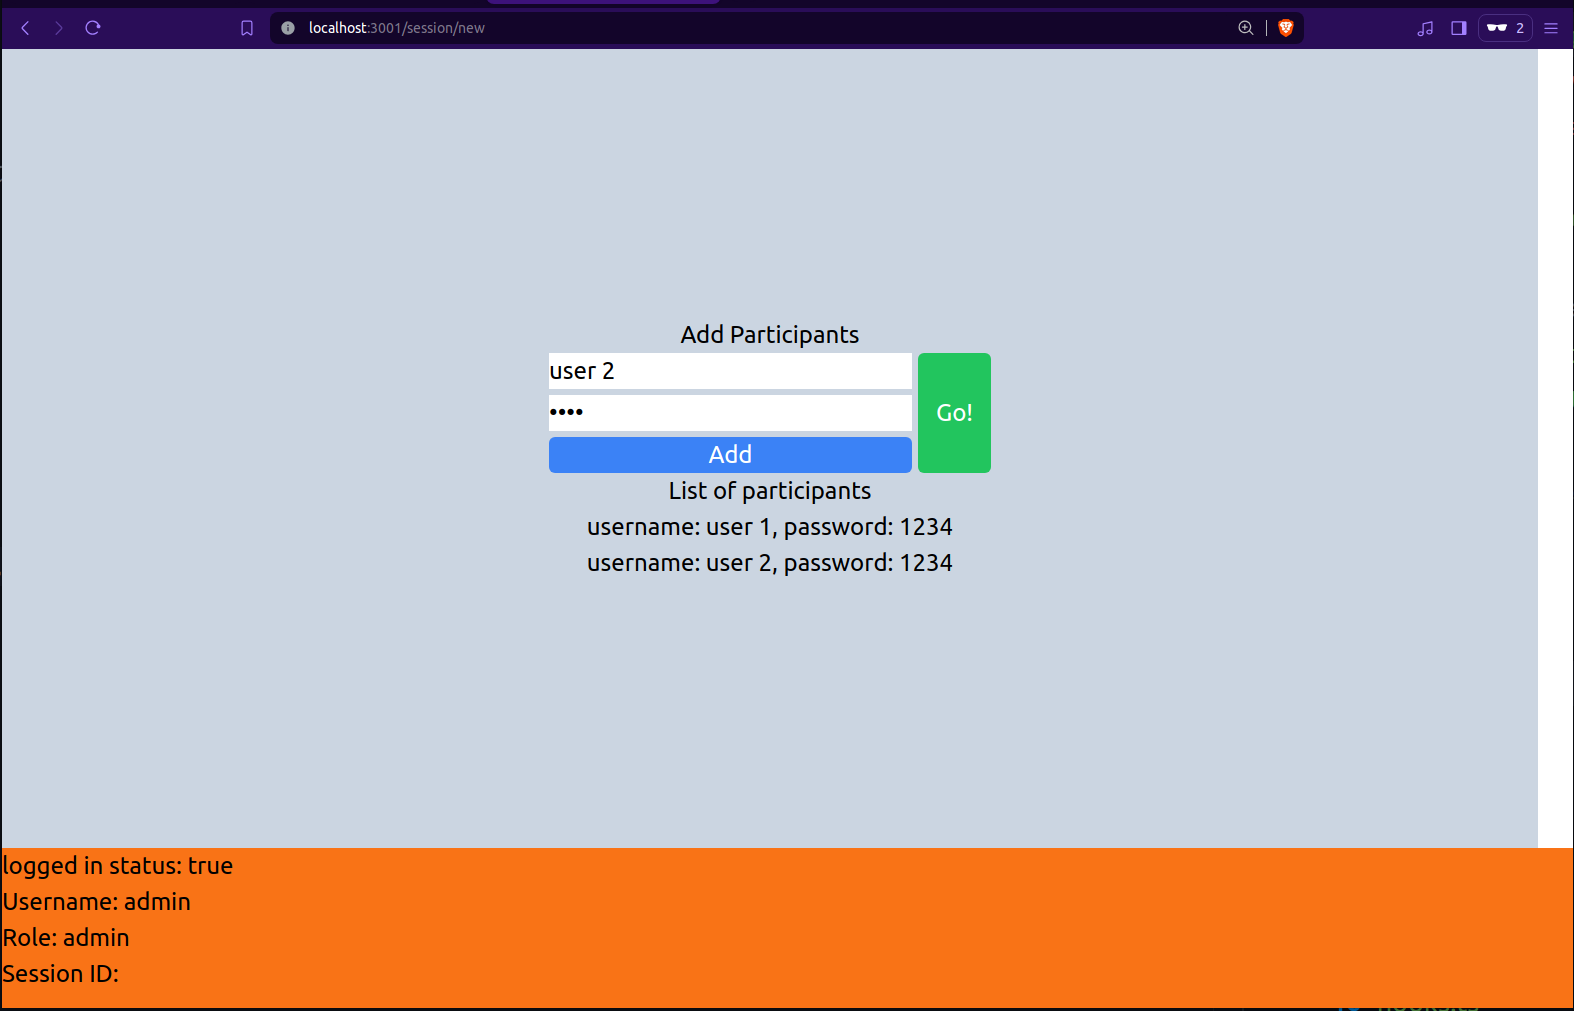
\includegraphics[width=0.8\textwidth]{diagrams/ChatroomNewSession.png}
    \caption{React Chatroom: Creating new session}
    \label{fig:enter-label}
\end{figure}

After creating the session by clicking the ‘Go!’ button, the admin will be redirected to the chatroom and other users can log in using the generated URL.

Other participants can join the session by entering the credentials provided by the admin and will be redirected to the chatroom.

Lastly, all users upon login will see the chat history and send new messages.

\begin{figure}[H]
    \centering
    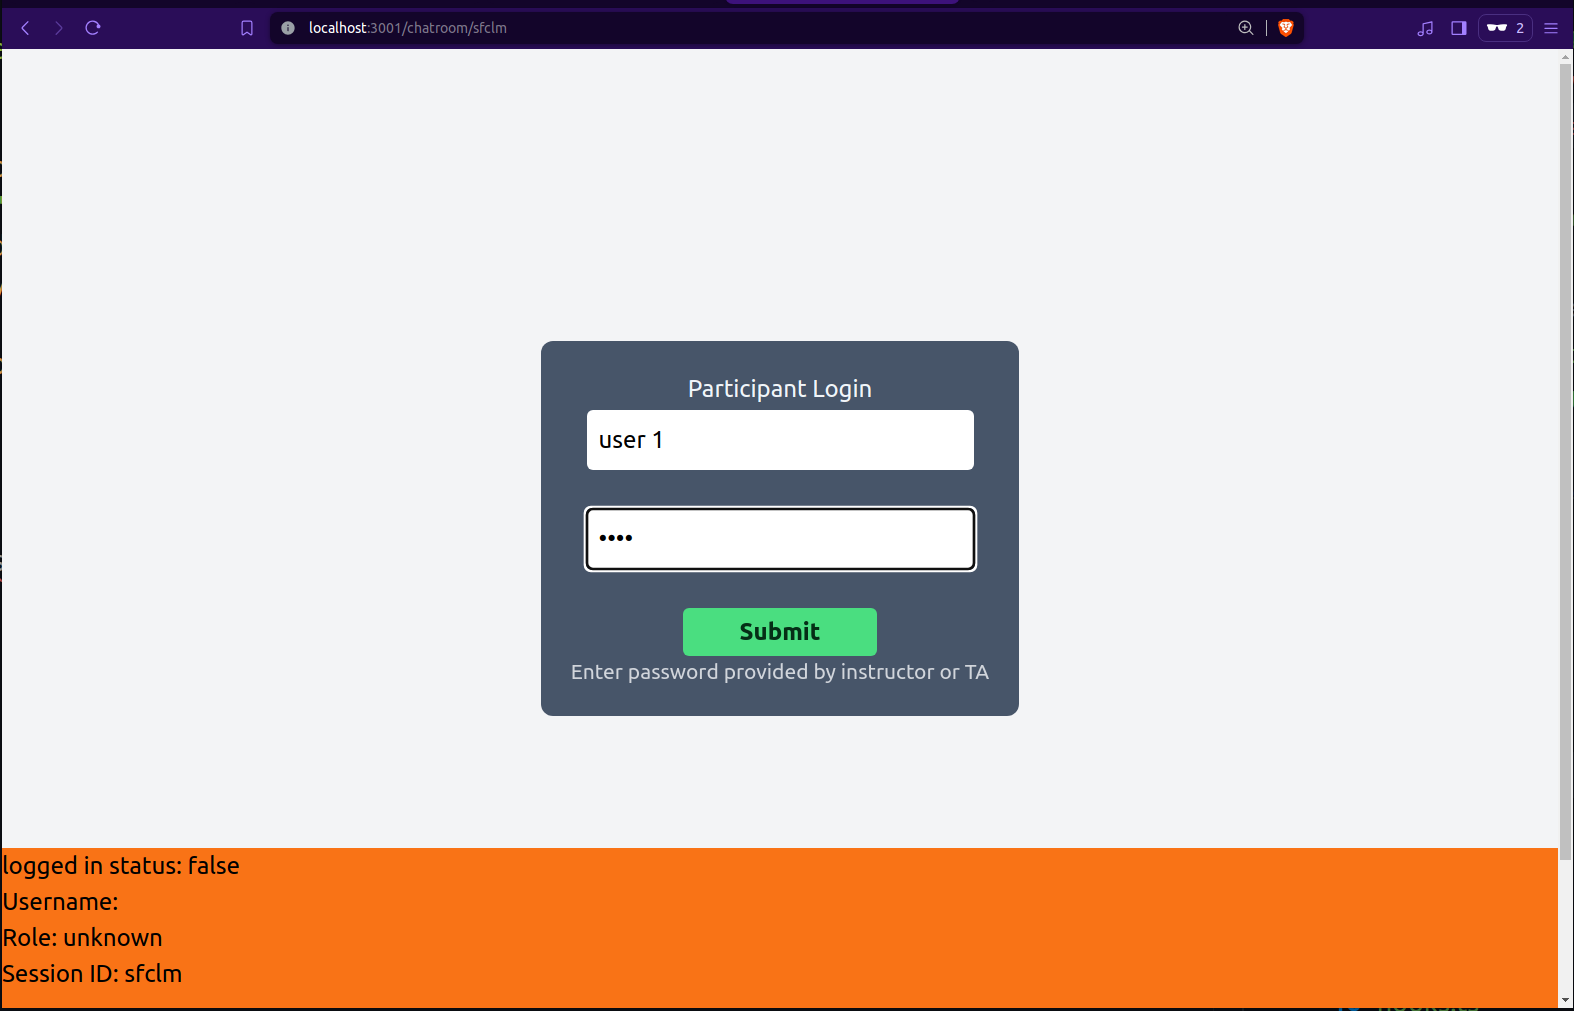
\includegraphics[width=0.8\textwidth]{diagrams/ChatroomUserLogin.png}
    \caption{React Chatroom: User login page}
    \label{fig:enter-label}
\end{figure}

\begin{figure}[H]
    \centering
    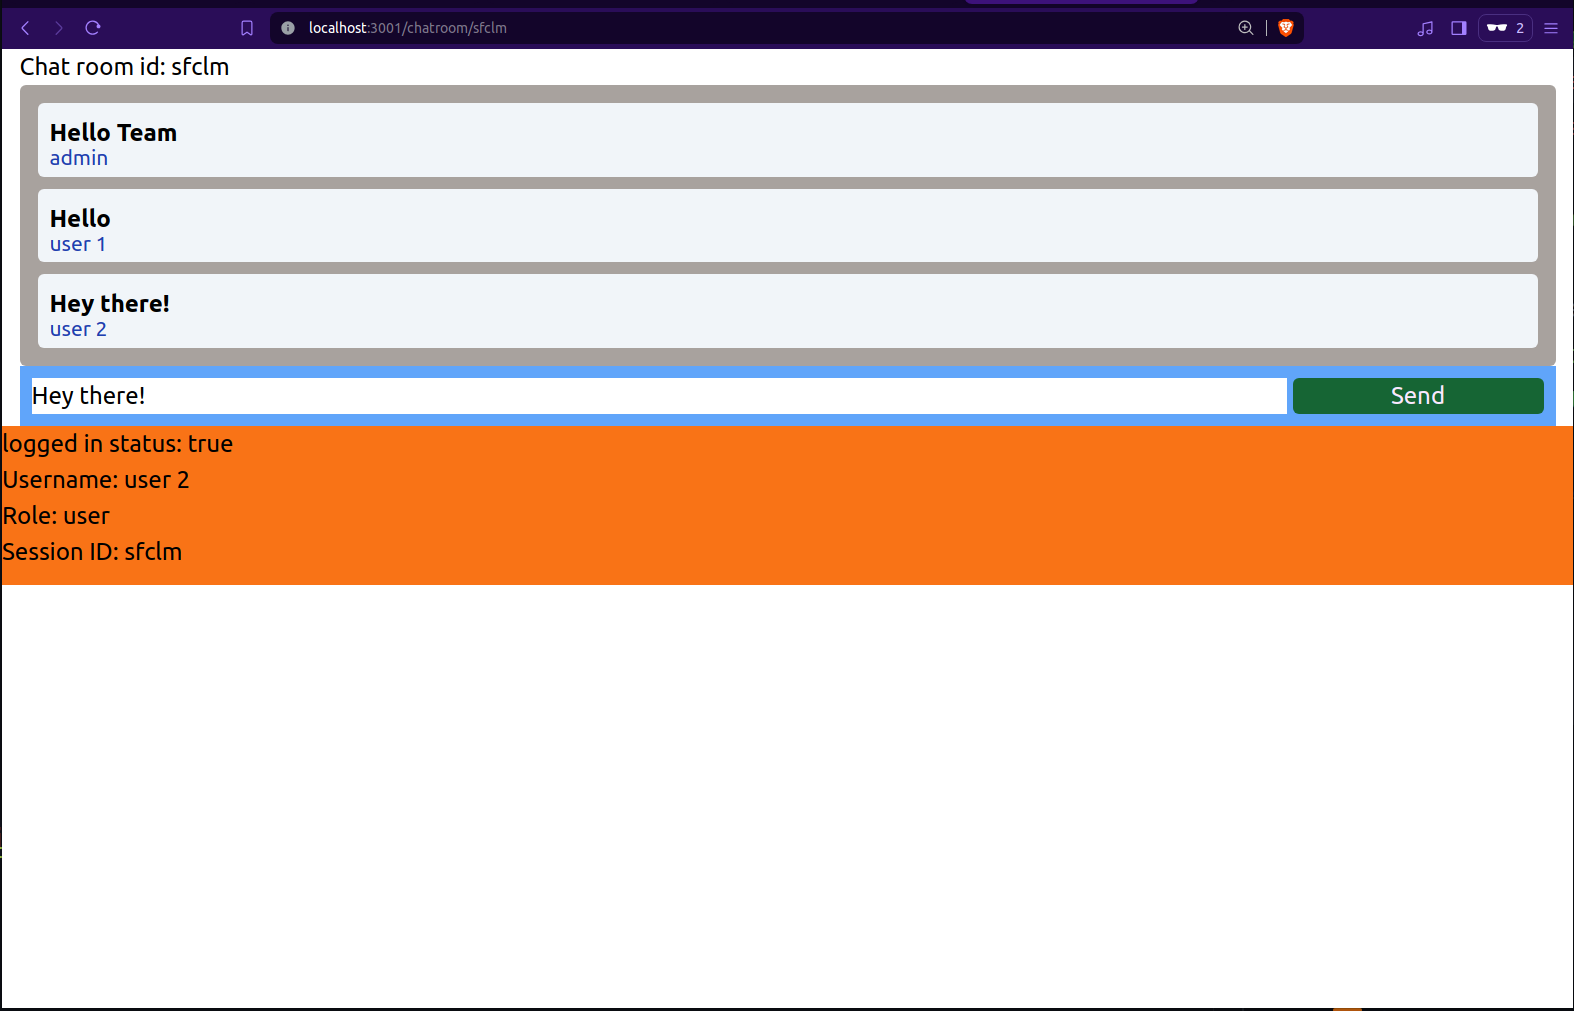
\includegraphics[width=0.8\textwidth]{diagrams/ChatroomMain.png}
    \caption{React Chatroom: Chat View Room}
    \label{fig:enter-label}
\end{figure}

\section{Calendar-Sync}

\textbf{TEASync}

\begin{figure}[H]
    \centering
    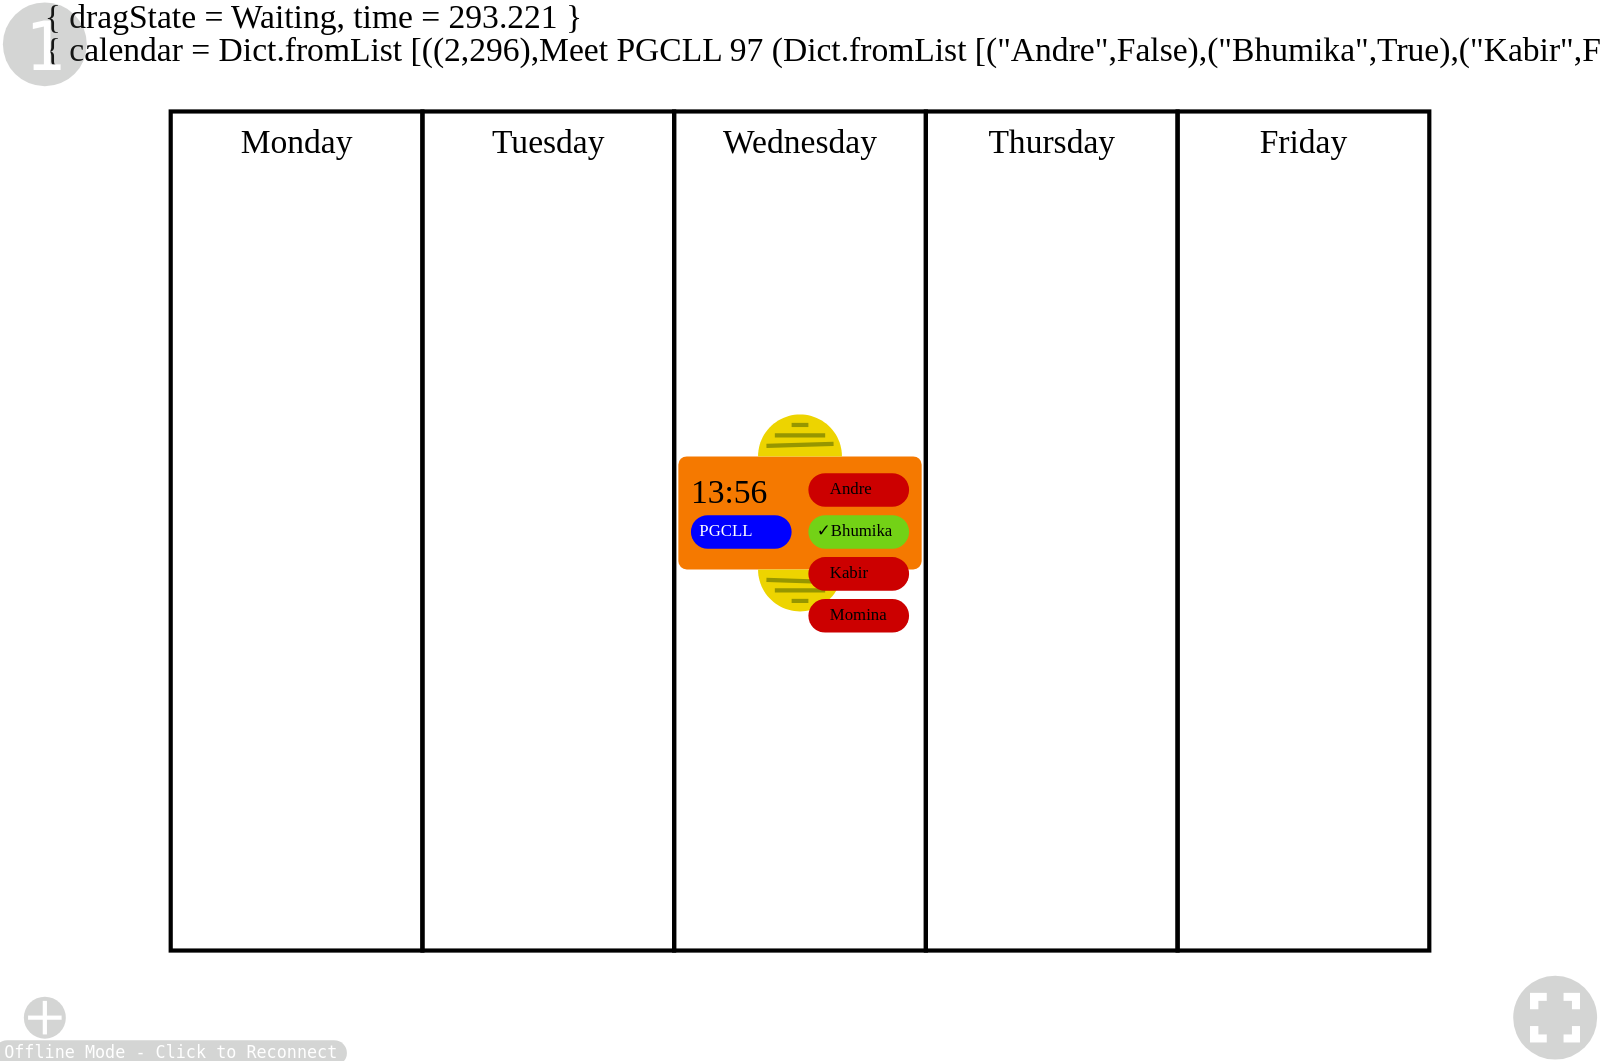
\includegraphics[width=0.8\textwidth]{diagrams/TEASyncCalendarApp.png}
    \caption{TEASync Calendar: Main View}
    \label{fig:enter-label}
\end{figure}


\textbf{React}

The homepage screen allows users to create or join any existing session.

\begin{figure}[H]
    \centering
    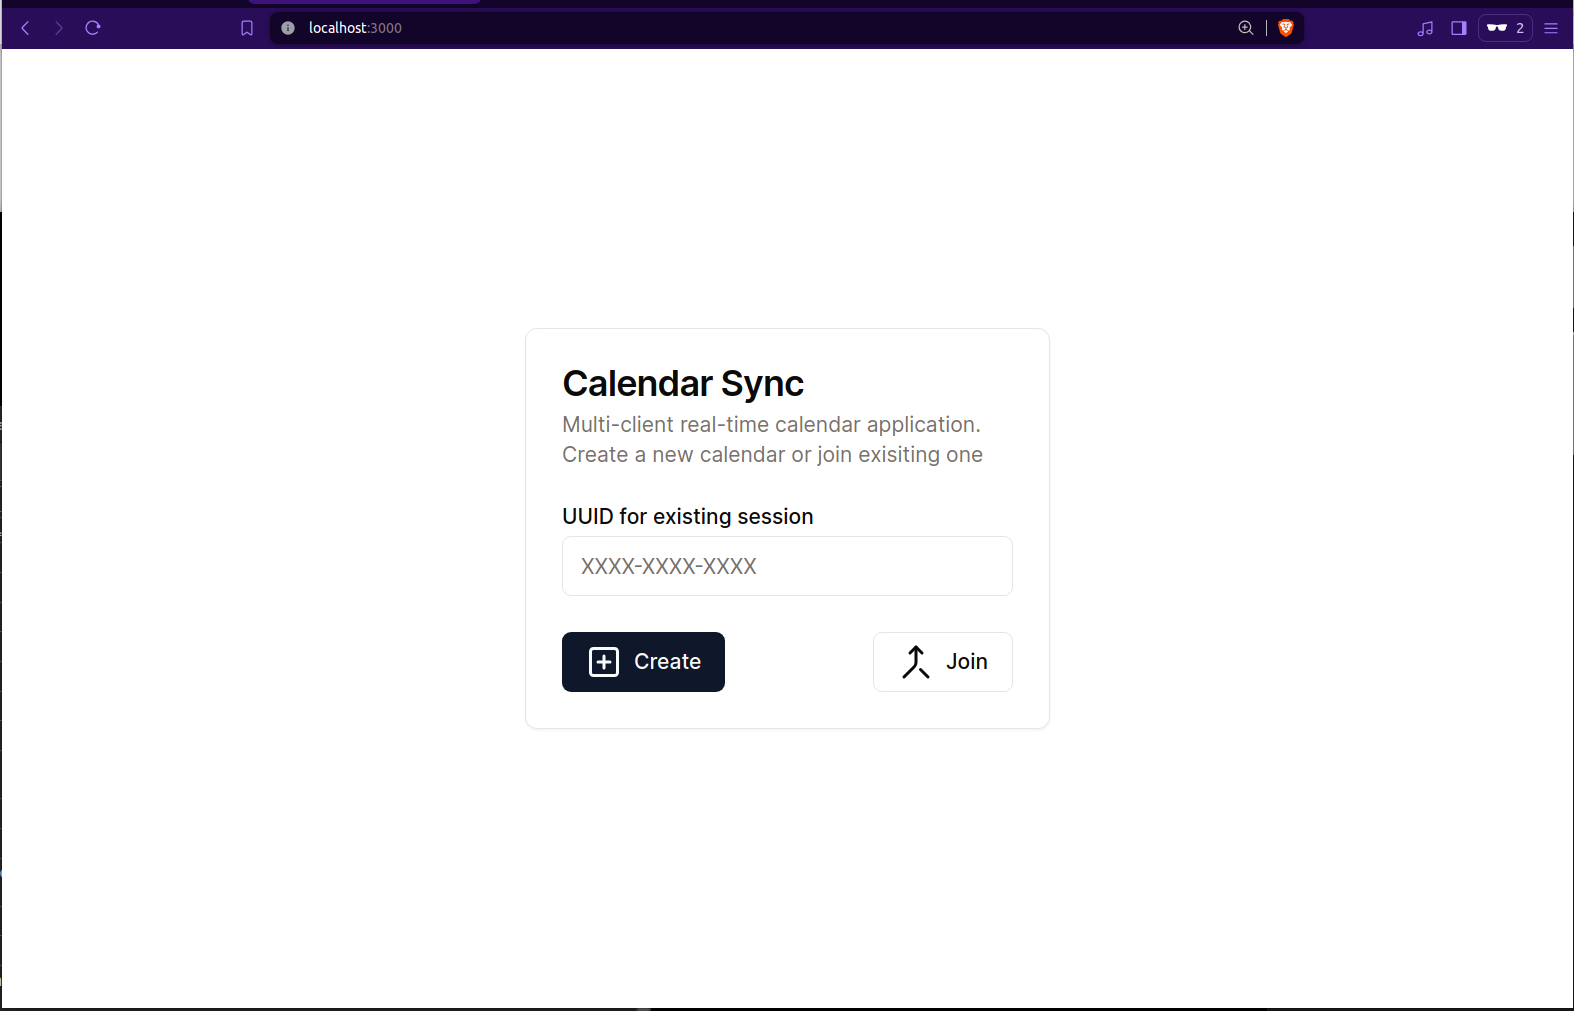
\includegraphics[width=0.8\textwidth]{diagrams/CalendarAppLogin.png}
    \caption{React Calendar: Login Page}
    \label{fig:enter-label}
\end{figure}

Choosing any of the options, the user will be redirected to the calendar view page, and they will see existing events, if any. 

In order to create a new event, users can double click on a slot on the calendar, and the system will present them with a dialog box to enter the event details.

\begin{figure}[H]
    \centering
    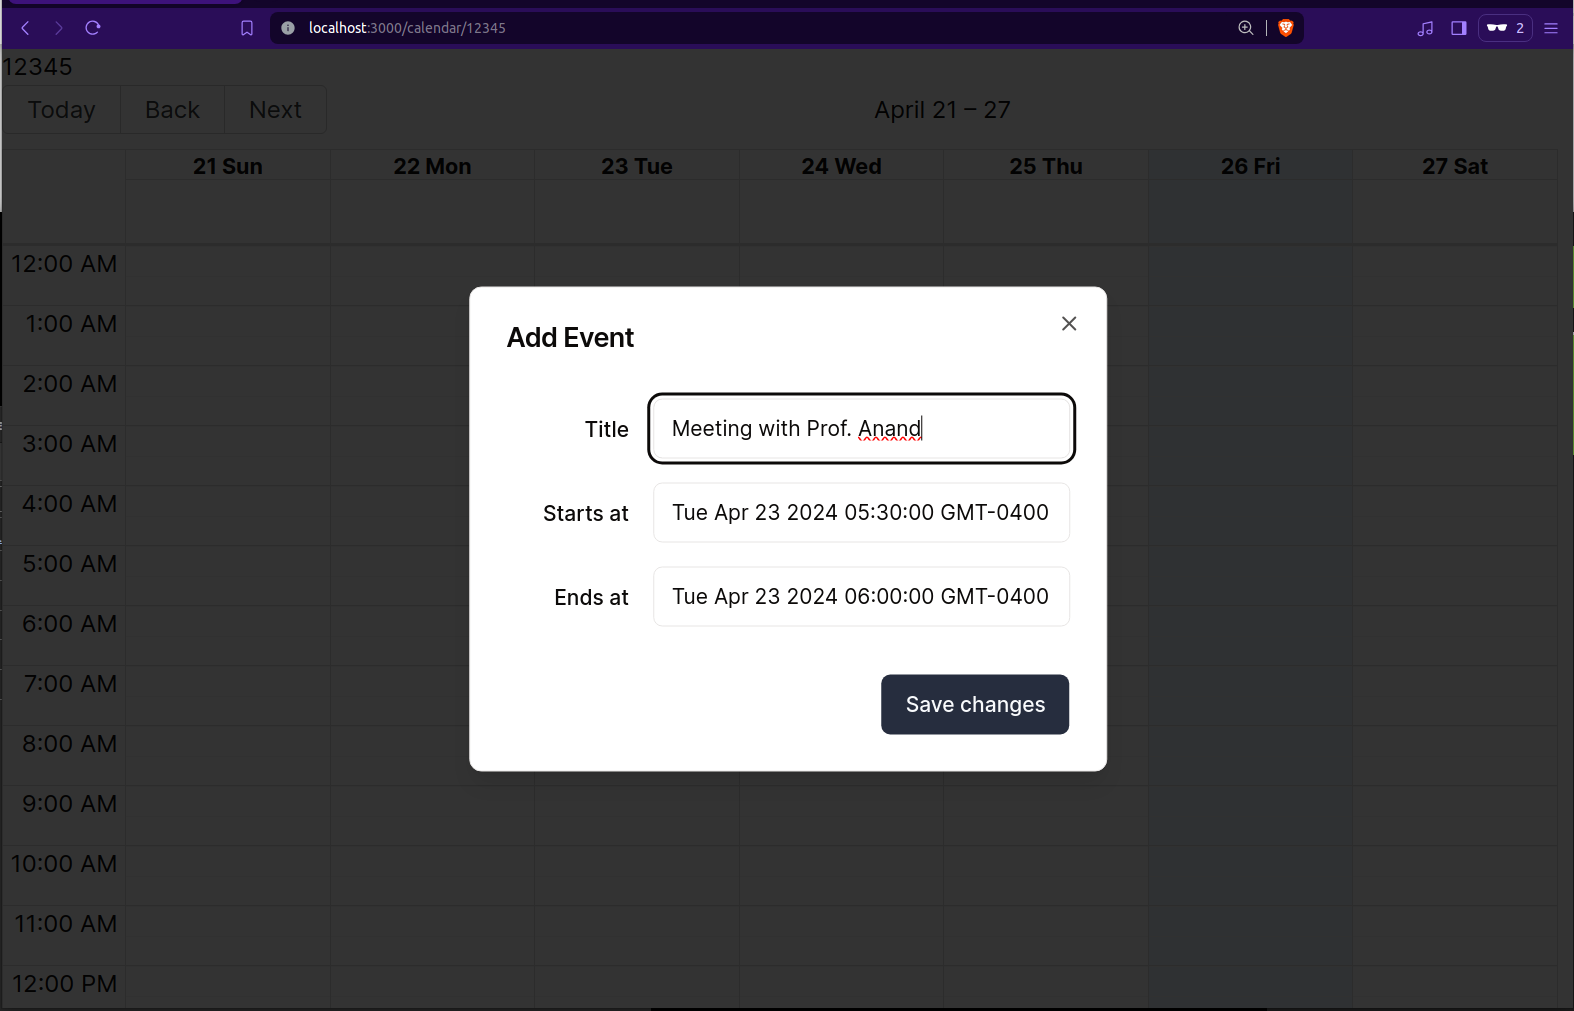
\includegraphics[width=0.8\textwidth]{diagrams/CalendarAppCreateEvent.png}
    \caption{React Calendar: New Event Input Dialog}
    \label{fig:enter-label}
\end{figure}

After saving changes, the event will be added to the calendar and will be reflected to all connected clients.

\begin{figure}[H]
    \centering
    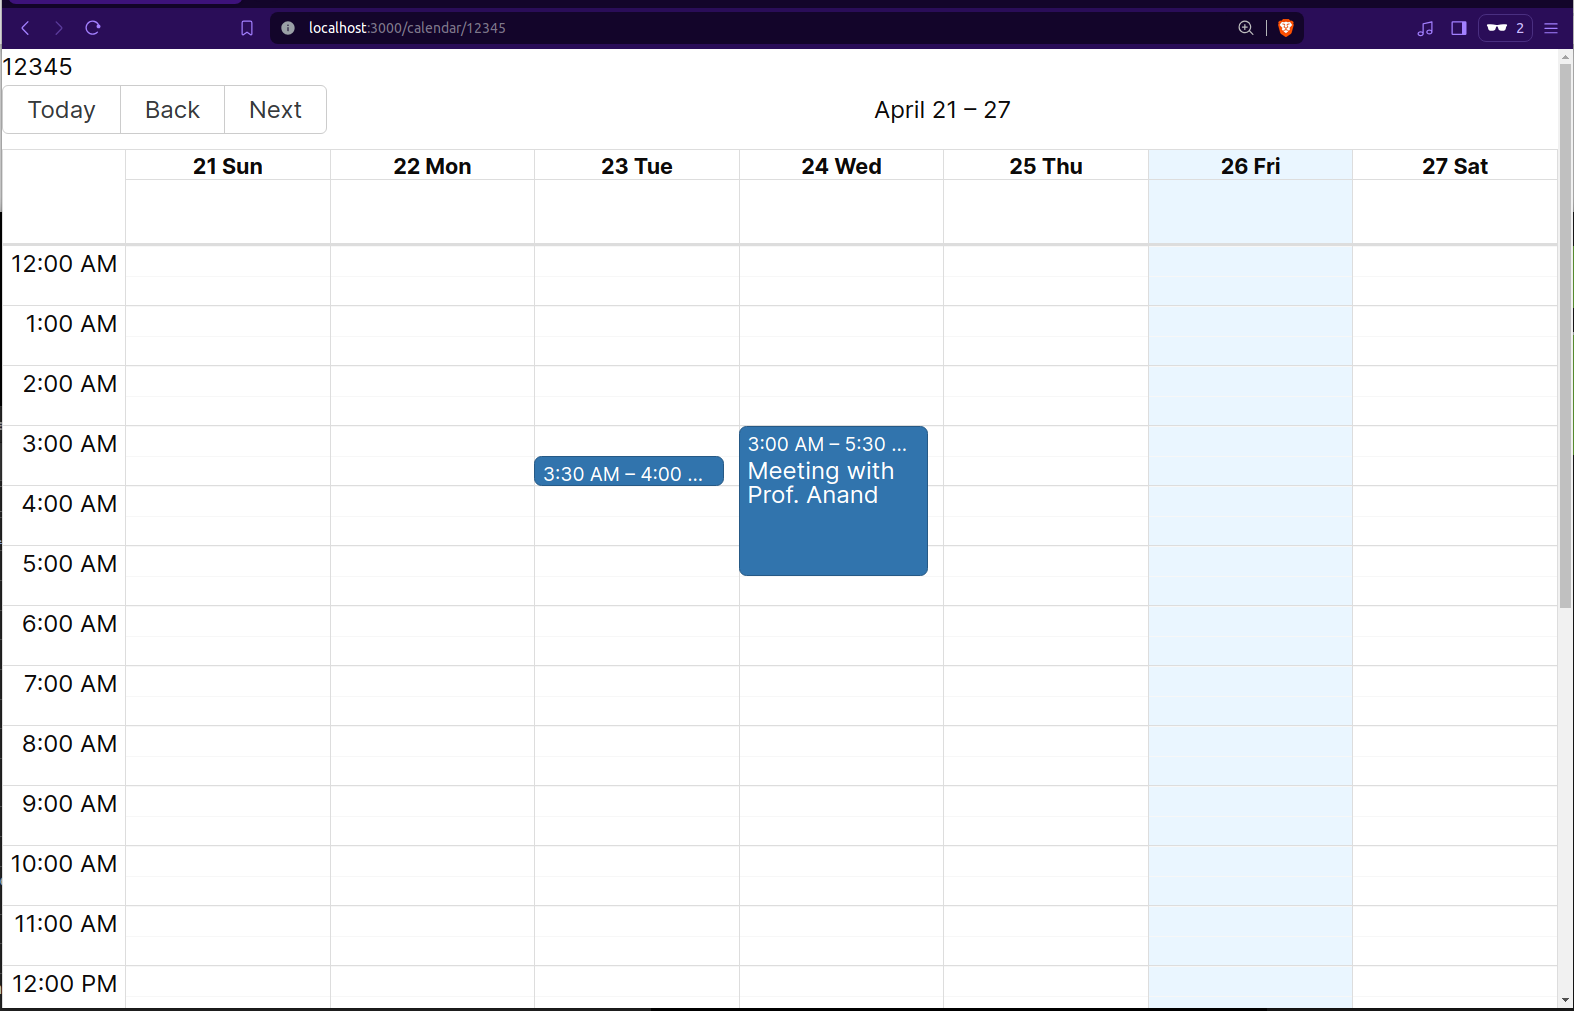
\includegraphics[width=0.8\textwidth]{diagrams/CalendarAppMain.png}
    \caption{React Calendar: Calendar View Page}
    \label{fig:enter-label}
\end{figure}
%----------------------------------------

% \blindtext[1]

% \begin{figure}[ht]
%     \centering
%     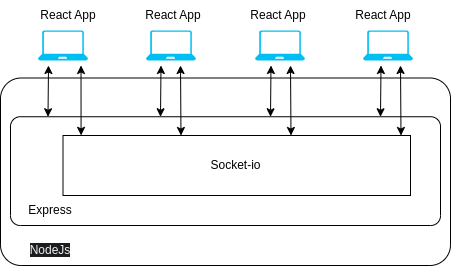
\includegraphics[width=0.8\textwidth]{diagrams/App Architecture.png}
%     \caption{Caption}
%     \label{fig:enter-label}
% \end{figure}